\documentclass[11pt]{article}
\usepackage{amssymb,amsmath,amsthm,latexsym,mathrsfs,array,amssymb,amsmath,epsfig,sudoku,amssymb,amsbsy,array,color,amssymb,amsmath,epsfig,sudoku,url}
\usepackage{minted}
\usepackage{pdflscape}
\usemintedstyle{vs}
\usepackage{booktabs}
\usepackage{float}

\usepackage{amsmath} % For advanced math features like \text, \frac, etc.
\usepackage[utf8]{inputenc} % To handle various characters
\usepackage{float}
\usepackage{booktabs}
%\usepackage[a4paper, margin=0.5in]{geometry}

\textheight 8.5in
\textwidth 6.25in
\voffset= -.55in
\hoffset= -.55in

\date{}
\pagestyle{empty}
\begin{document}
%\begin{landscape}
%\thispagestyle{empty}
\begin{center} {\LARGE\textbf{{CSCI 6360}}}\end{center}
\begin{center}{\Large \textbf{Project 3}}\end{center}
%\begin{center}{Masum Billah \\ University of GA \\ Department of Statistics}\end{center}       
\begin{center} \date{\today} \today \end{center}
    
\vspace{.1in}

\section{Random Forest Performance on Dataset 2}

The Random Forest model was trained and evaluated on both in-sample and out-of-sample data. Hyperparameter tuning was performed using cross-validation on the training set to determine the optimal parameters. The tuning process considered the following parameters:

\begin{minted}{python}
params = {
    'n_estimators': [200, 300, 400, 500, 700],
    'max_depth': [10, 20, 30, None],
    'min_samples_split': [2, 5, 10],
    'min_samples_leaf': [1, 2, 4],
    'max_features': ['sqrt', 'log2', 0.5],
    'bootstrap': [True, False]
}
\end{minted}

\section{In-Sample Quality of Fit Metrics}

\begin{table}[h]
\centering
\caption{In-sample performance metrics of the Random Forest model.}
\begin{tabular}{lc}
\hline
Metric & Value \\
\hline
$R^2$ & 0.9549 \\
SST & 9.78$\times 10^{11}$ \\
SSE & 4.41$\times 10^{10}$ \\
MSE & 441081.88 \\
RMSE & 664.14 \\
MAE & 374.50 \\
$m$ & 100000 \\
\hline
\end{tabular}
\end{table}

\begin{figure}[h]
\centering
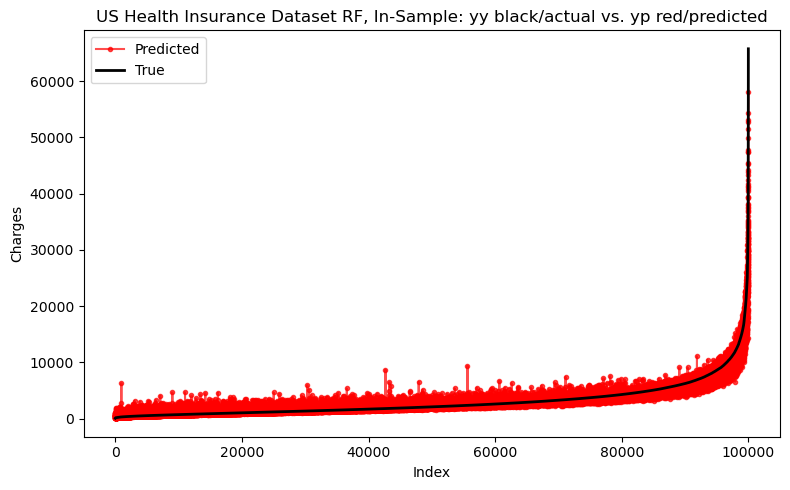
\includegraphics[width=0.9\textwidth]{figure/rf21.jpg}
\caption{In-sample performance of the Random Forest model on Dataset 2.}
\label{fig:RF1}
\end{figure}
\clearpage

\section{Out-of-Sample Quality of Fit Metrics}
\begin{table}[h]
\centering
\caption{Out-of-sample performance metrics of the Random Forest model.}
\begin{tabular}{lc}
\hline
Metric & Value \\
\hline
$R^2$ & 0.6510 \\
SST & 1.97$\times 10^{11}$ \\
SSE & 6.87$\times 10^{10}$ \\
MSE & 3434098.68 \\
RMSE & 1853.13 \\
MAE & 1025.39 \\
$m$ & 20000 \\
\hline
\end{tabular}
\end{table}

\begin{figure}[h]
\centering
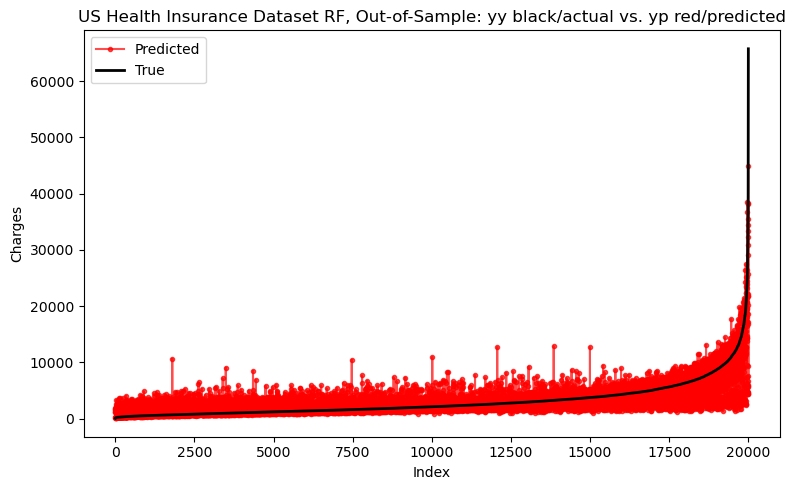
\includegraphics[width=0.9\textwidth]{figure/rf22.jpg}
\caption{Out-of-sample performance of the Random Forest model on Dataset 2.}
\label{fig:RF2}
\end{figure}
\newpage

\section{Fine-Tuned Quality of Fit Metrics}
A total of 20 hyperparameter configurations were randomly sampled, and each was evaluated using 5-fold cross-validation. The following parameter settings were identified as optimal:
\begin{minted}{python}
Best params: {'n_estimators': 300, 
'min_samples_split': 5, 'min_samples_leaf': 4,
'max_features': 0.5, 'max_depth': None, 
'bootstrap': False}
\end{minted}

\begin{table}[h]
\centering
\caption{Fine-tuned performance metrics of the Random Forest model.}
\begin{tabular}{lc}
\hline
Metric & Value \\
\hline
$R^2$ & 0.6542 \\
SST & 1.97$\times 10^{11}$ \\
SSE & 6.80$\times 10^{10}$ \\
MSE & 3402240.89 \\
RMSE & 1844.52 \\
MAE & 999.62 \\
$m$ & 20000 \\
\hline
\end{tabular}
\end{table}


\begin{figure}[h]
\centering
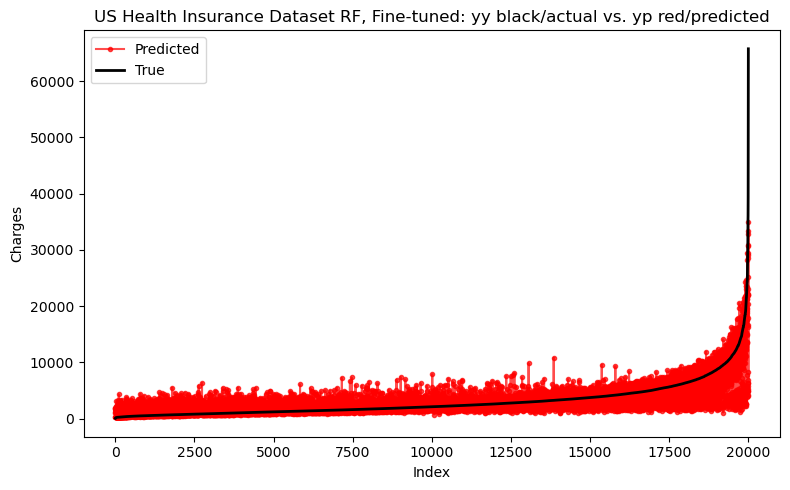
\includegraphics[width=0.9\textwidth]{figure/rf23.jpg}
\caption{Fine-tuned performance of the Random Forest model on Dataset 2.}
\label{fig:RF3}
\end{figure}
\newpage

\section{Feature Importance from the Best-Performing Model}

\begin{figure}[h]
\centering
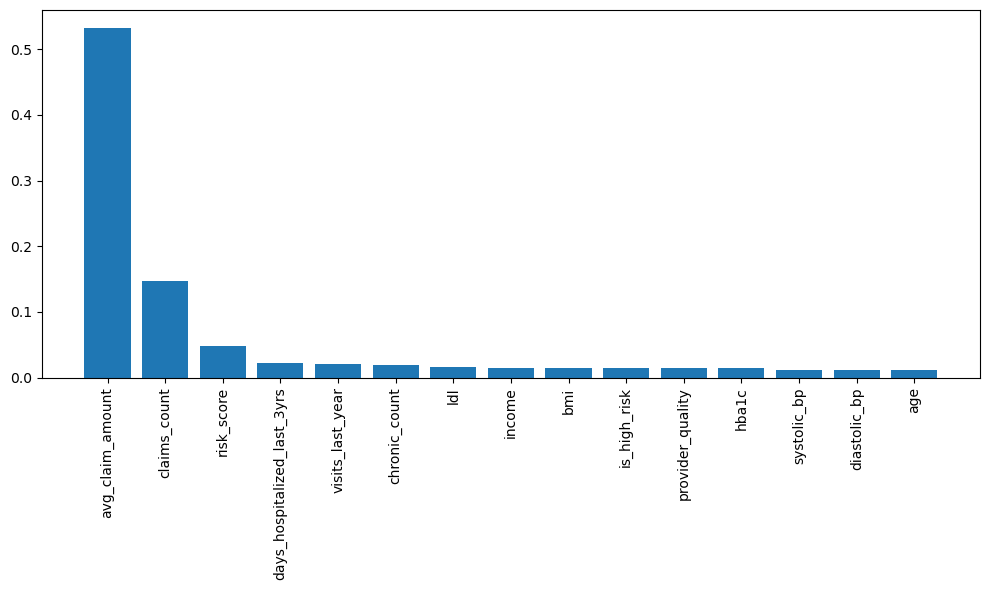
\includegraphics[width=0.9\textwidth]{figure/rf24.jpg}
\caption{Top 15 Most Important Features.}
\label{fig:RF4}
\end{figure}
\end{document}